%\begin{figure}[t]
%\vspace{-0.5in}
%\centering
%\psfig{figure=figures/plots/runtimeFinal.eps,width=5.5in} }
%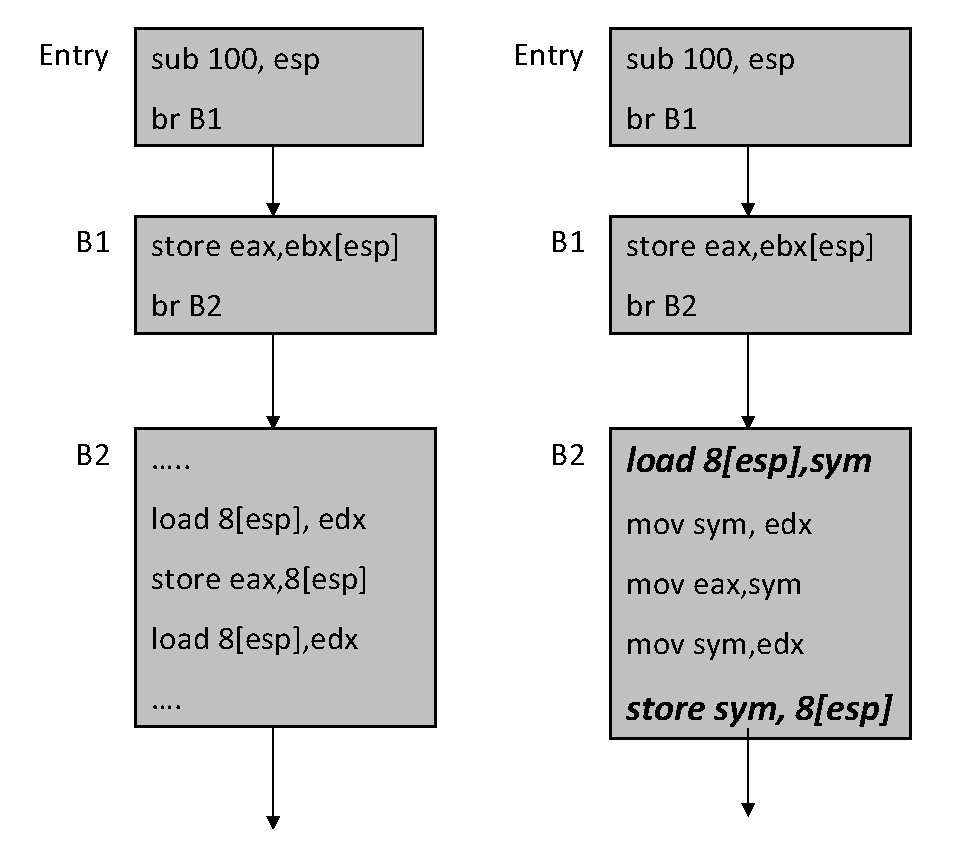
\includegraphics [width=0.5\linewidth] {figures/EPS/cfgex.eps} 
%\tiny{
%\caption { \textit{Stack layout in a binary}}
%}
%\label{fig:stack-layout}
%\end{figure}

\begin{figure}[t]
{
%\begin{minipage}{.5\linewidth}
{
\centering
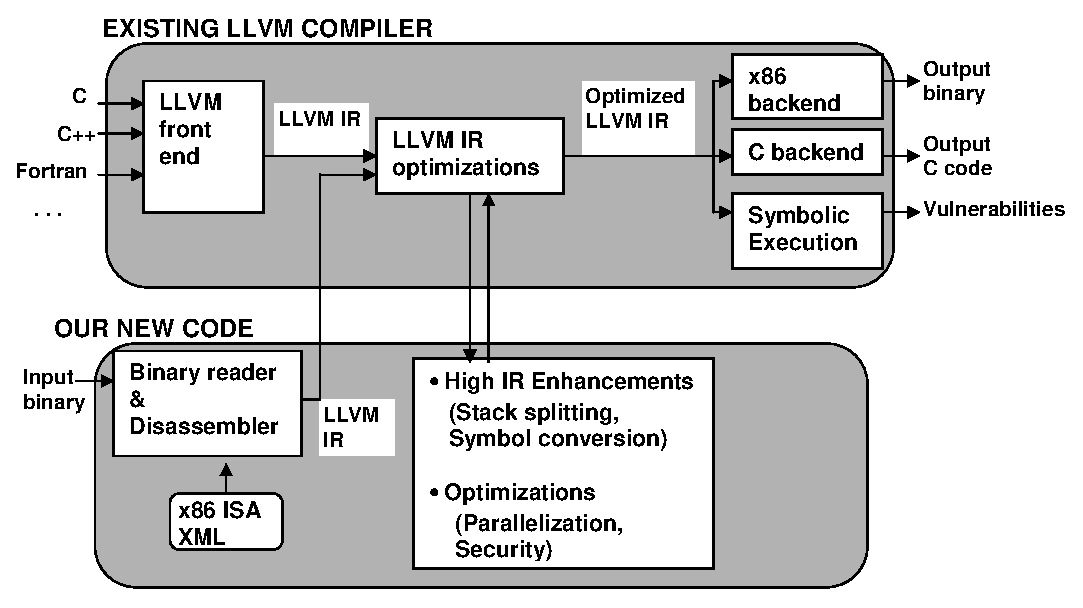
\includegraphics[width=0.7\linewidth]{figures/EPS/flow1.eps}
\caption{\scriptsize{System Flow}}
\label{fig:systemflow}
\vspace{-0.2in}
}
%\end{minipage}
\hfill
%\begin{minipage}{0.3\linewidth}
%{
%\centering
%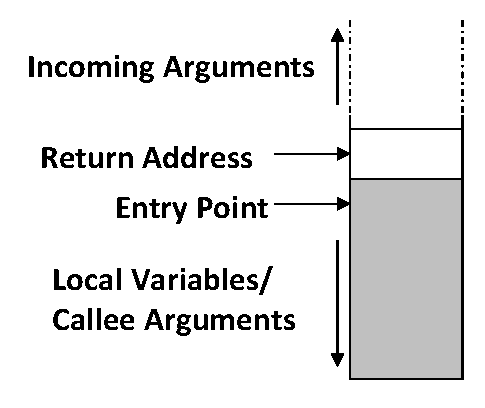
\includegraphics[width=\linewidth]{figures/EPS/stackLayout1.eps} 
%\caption{A typical stack layout}
%\label{fig:stacklayout}
%}
%\end{minipage}
\vspace{-0.2in}
}
\end{figure}
